\documentclass[a4paper,12pt]{article}
\usepackage[T1]{fontenc}
\usepackage[utf8]{inputenc}
\usepackage{graphicx}

\title{\texttt{oubliette} user stories}
\author{Starship Troopers}
\date{\today}

\begin{document}
\maketitle

\begin{abstract}
\texttt{oubliette} is a text-based role-playing game in the style of
video games that were prevalent in the 1960s and 1970s. It's designed
to provide relief to busy workers in their downtime as well as attracting
interest from the lucrative video game market.
\end{abstract}

\section{Background}
It's quite easy for the scope and ambition of a video game project to
quickly outstrip both time and budgetary constraints. Therefore, the team
agreed from the outset to aggressively limit the size of the project to
the bare essentials. For \texttt{oubliette}, this meant prioritising the
following over-arching features:

\begin{enumerate}
\item Dynamic character creation
\item Semantic dungeon navigation
\item Combat
\item A fleshed-out world
\end{enumerate}

\section{Feature sizing}
The next task we tackled as a team is assigning sizes to each of our
user stories. To facilitate group discussion and decision-making on user
story sizes, the team performed a period of cursory research to identify
an agile-focused software tool.

The team quickly decided on an Android application called
``Radtac Agile Tools'', which provides a simple and intuitive card-based
user-interface for displaying individual user story sizes (see Figure 1).

Subsequent to our stand-up meeting on the 5th of February, the team
engaged in the process of estimating the relative sizes for our user
stories. The Radtac tool's visual element enabled us to rapidly iterate
through our user stories and assign unanimous estimates to them.

As we had anticipated, there was several differences in opinions in
regards to the user story sizes. However, as per our team agreement,
we calmly and honestly discussed our opposing points-of-view and
within the hour we had sized all of our user stories with the aid of
the Radtac tool.

\begin{figure}[h]
\caption{\textit{Radtac Agile Tools}}
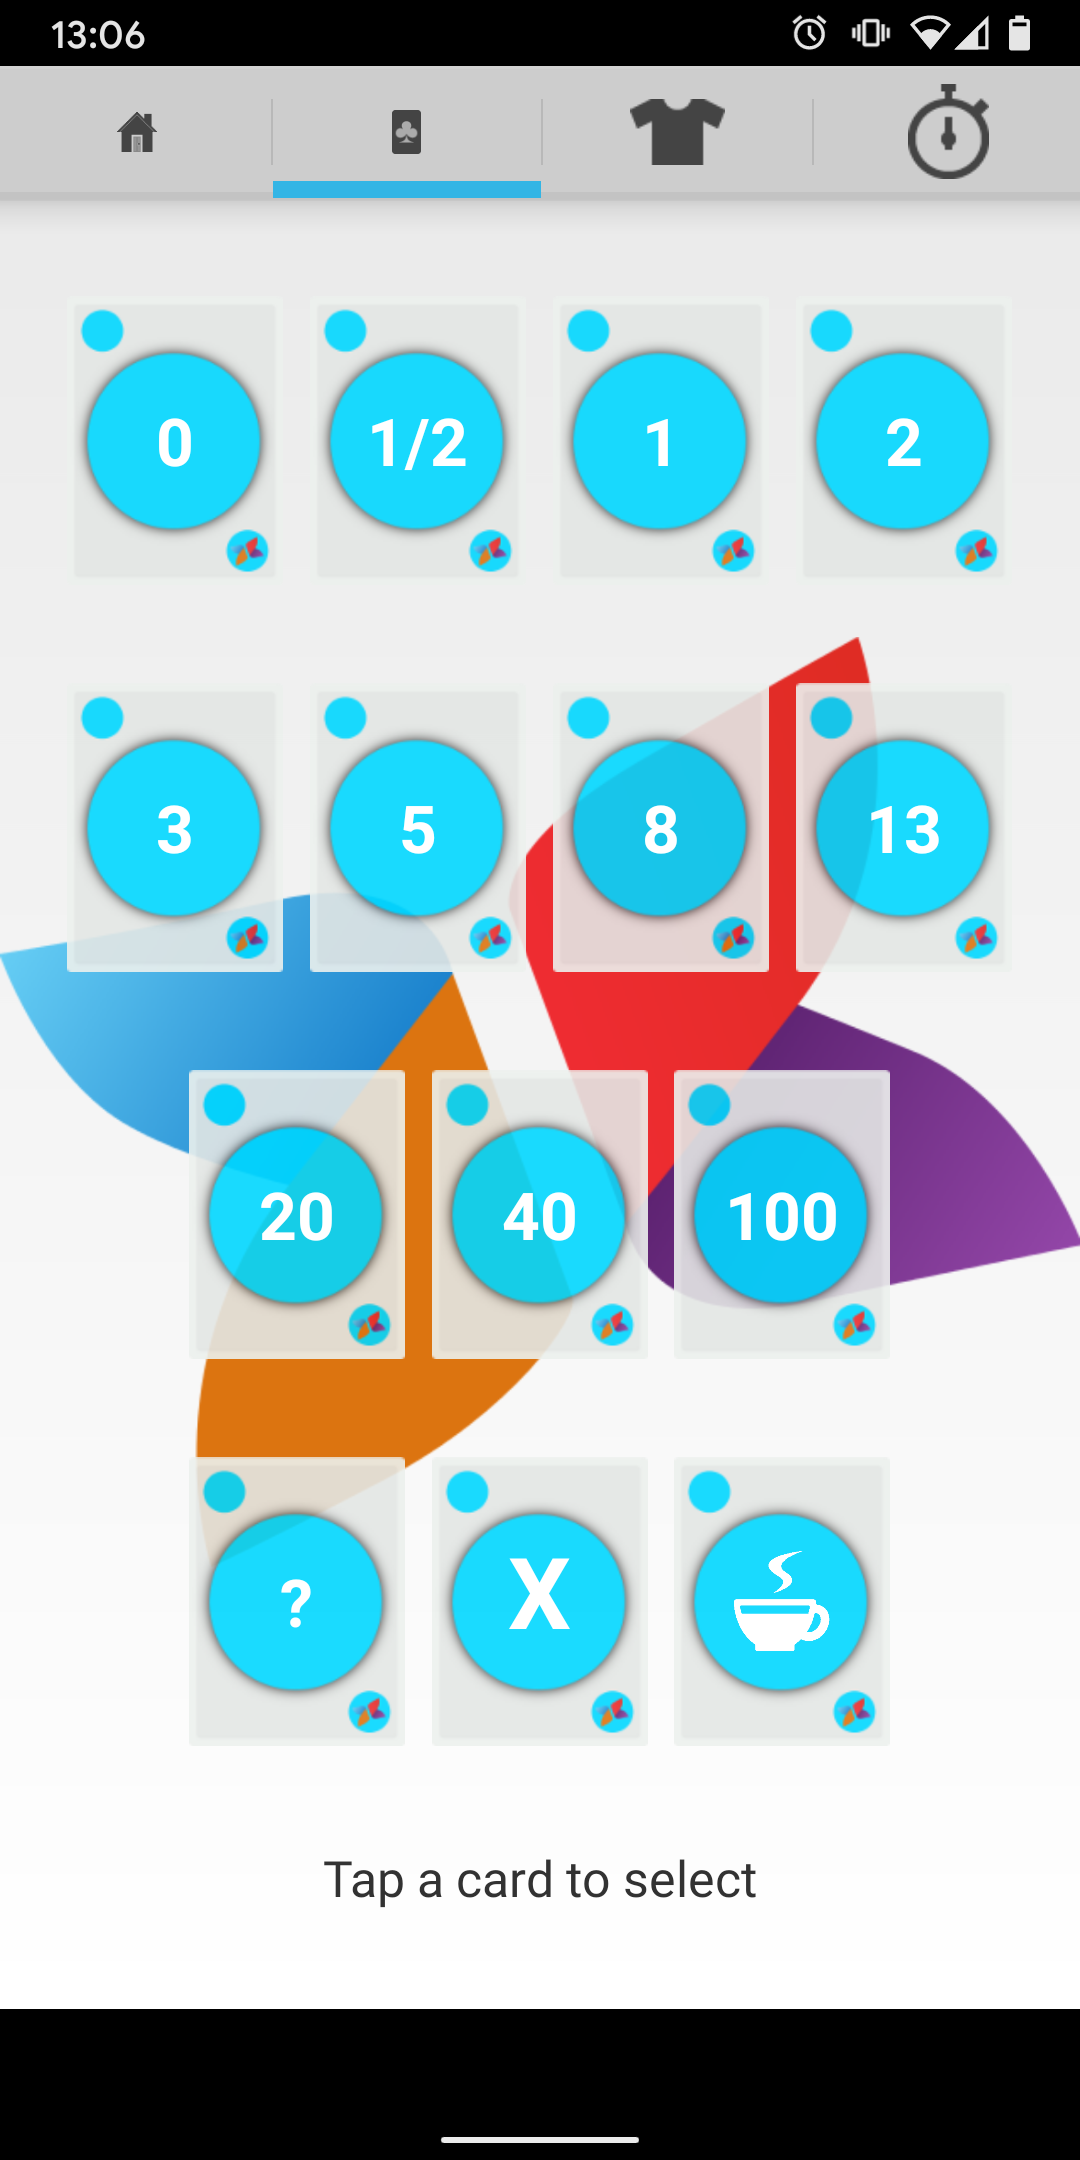
\includegraphics[scale=0.15]{radtac}
\centering
\end{figure}


\end{document}